\documentclass[a4paper,11pt]{article}
\usepackage{amsmath,amsthm,amsfonts,amssymb,amscd,amstext,vmargin,graphics,graphicx,tabularx,multicol} 
\usepackage[francais]{babel}
\usepackage[utf8]{inputenc}  
\usepackage[T1]{fontenc} 
\usepackage{pstricks-add,tikz,tkz-tab,variations}
\usepackage[autolanguage,np]{numprint} 

\setmarginsrb{1.5cm}{0.5cm}{1cm}{0.5cm}{0cm}{0cm}{0cm}{0cm} %Gauche, haut, droite, haut
\newcounter{numexo}
\newcommand{\exo}[1]{\stepcounter{numexo}\noindent{\bf Exercice~\thenumexo} : \marginpar{\hfill /#1}}
\reversemarginpar


\newcounter{enumtabi}
\newcounter{enumtaba}
\newcommand{\q}{\stepcounter{enumtabi} \theenumtabi.  }
\newcommand{\qa}{\stepcounter{enumtaba} (\alph{enumtaba}) }
\newcommand{\initq}{\setcounter{enumtabi}{0}}
\newcommand{\initqa}{\setcounter{enumtaba}{0}}

\newcommand{\be}{\begin{enumerate}}
\newcommand{\ee}{\end{enumerate}}
\newcommand{\bi}{\begin{itemize}}
\newcommand{\ei}{\end{itemize}}
\newcommand{\bp}{\begin{pspicture*}}
\newcommand{\ep}{\end{pspicture*}}
\newcommand{\bt}{\begin{tabular}}
\newcommand{\et}{\end{tabular}}
\renewcommand{\tabularxcolumn}[1]{>{\centering}m{#1}} %(colonne m{} centrée, au lieu de p par défault) 
\newcommand{\tnl}{\tabularnewline}

\newcommand{\trait}{\noindent \rule{\linewidth}{0.2mm}}
\newcommand{\hs}[1]{\hspace{#1}}
\newcommand{\vs}[1]{\vspace{#1}}

\newcommand{\N}{\mathbb{N}}
\newcommand{\Z}{\mathbb{Z}}
\newcommand{\R}{\mathbb{R}}
\newcommand{\C}{\mathbb{C}}
\newcommand{\Dcal}{\mathcal{D}}
\newcommand{\Ccal}{\mathcal{C}}
\newcommand{\mc}{\mathcal}

\newcommand{\vect}[1]{\overrightarrow{#1}}
\newcommand{\ds}{\displaystyle}
\newcommand{\eq}{\quad \Leftrightarrow \quad}
\newcommand{\vecti}{\vec{\imath}}
\newcommand{\vectj}{\vec{\jmath}}
\newcommand{\Oij}{(O;\vec{\imath}, \vec{\jmath})}
\newcommand{\OIJ}{(O;I,J)}


\newcommand{\bmul}[1]{\begin{multicols}{#1}}
\newcommand{\emul}{\end{multicols}}

\newcommand{\reponse}[1][1]{%
\multido{}{#1}{\makebox[\linewidth]{\rule[0pt]{0pt}{20pt}\dotfill}
}}

\newcommand{\titre}[5] 
% #1: titre #2: haut gauche #3: bas gauche #4: haut droite #5: bas droite
{
\noindent #2 \hfill #4 \\
#3 \hfill #5

\vspace{-1.6cm}

\begin{center}\rule{6cm}{0.5mm}\end{center}
\vspace{0.2cm}
\begin{center}{\large{\textbf{#1}}}\end{center}
\begin{center}\rule{6cm}{0.5mm}\end{center}
}



\begin{document}
\pagestyle{empty}
\titre{Contrôle 5}{Nom :}{Prénom :}{Classe}{Date}



\exo{3,5}  Calculer les expressions suivantes en écrivant les étapes de vos calculs :\\

\bmul{3}

$P = 2 + (4 \times 5)^{2}$

\columnbreak

$E = 5 - 3 \times (-2)^{3}$

\columnbreak

$M = 3(1-3)^{2} - 2^{7} \times (3^{0} - 2)$\\

\emul

\exo{3,5} Donner les résultats sous la forme d'une seule puissance.

\bmul{3}

$ L = 11^{6} \times 11^{-5} \times 11^{10}$\\

$ G = \dfrac{(-5)^{1}}{(-5)^{4}} $\\

\columnbreak

$ V = \dfrac{10^{0} \times 10^{-1}}{10^{-2}}  $\\

$ I = 3^{5} \times 8^{5} $\\

\columnbreak

$ R = \dfrac{10^{4}}{5^{4}} $\\

$ A = \dfrac{7^{-1} \times 7^{3} \times (7^{2})^{3}}{7^{5}} $\\

\emul


\exo{3,5} Donner l'écriture scientifique de chaque nombre. 

\bmul{4}

\begin{flushleft}
$B = 5 324,69 $
\end{flushleft}

\columnbreak

\begin{flushleft}
$Z = 0,000051 $
\end{flushleft}

\columnbreak

\begin{flushleft}
$ H = 768,79 \times 10^{-4}$
\end{flushleft}

\columnbreak

$ D = \dfrac{0,3 \times 10^{2} \times 5 \times 10^{-3}}{4 \times 10^{-4}}$\\

\emul

\exo{1}Voici l'éloignement par rapport à la Terre de plusieurs étoiles.

\bmul{2}

\begin{tabular}{|c|c|}
\hline 
Véga & $2,5 \times 10^{14} $ km \\ 
\hline 
Alpha du Centaure A & $4,2 \times 10^{13}$ km\\ 
\hline 
Arcturus & $34 \times 10^{13}$ km\\ 
\hline 
Canopus & $ 9,3 \times 10^{14} $ km\\ 
\hline 
Capella & $4,3 \times 10^{14} $ km\\ 
\hline 
Sirius & $82 \times 10^{12}$ km\\ 
\hline 
\end{tabular} 

Classer ces étoiles de la plus proche à la plus lointaine.

\columnbreak


\includegraphics[scale=1]{etoiles.eps} 

\emul

\exo{2,5}

\bmul{2}

\q Faire un schéma de l'escabeau en y reportant les longueurs données.\\

\q Quelle est la distance entre les pieds de cet escabeau ? (Justifier votre réponse)\\

\columnbreak

\includegraphics[scale=1]{escabeau.eps} 


\emul

\exo{3}

\bmul{2}

Les droites (UB) et (DS) sont parallèles ; NB = 6,5 cm ; UB = 9 cm et DS = 14,4 cm.

\initq \q Calculer la longueur NS. (Justifier votre réponse)\\

\q En déduire la longueur de BS.\\

\columnbreak

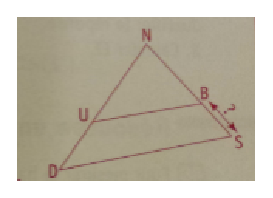
\includegraphics[scale=1]{triangle.eps} 

\emul


\exo{3}

Pour mesurer la hauteur de sa maison, Laurent vise le sommet de son toit et fait coïncider avec le haut de son muret. Voici un schéma de la situation.

\begin{center}
\includegraphics[scale=1]{maison.eps} 
\end{center}

Le muret a une hauteur de 1,30 m. Laurent (L) est à 4 m du muret et  la distance entre le centre de la maison et le muret est de 21 m.\\

\initq \q Faire un schéma en y reportant les longueurs données.\\

\q Déterminer, en justifiant, la hauteur de la maison.\\



\exo{} BONUS\\

\initq \q « Mille milliards de mille sabords !!!!!! ».  \\
Traduire cette phrase célèbre par une puissance de 10.\\

\q La masse de la Terre est de $5,9722 \times 10^{24}$ kg. Un petit grain de sable pèse $3 \times 10^{-9} $ kg.\\
Combien faudrait-il de grains de sable pour obtenir la masse de la Terre.\\

\q Le code secret d'une carte bleue est constitué de 4 chiffres. Combien de codes différents existe-t-il?



\end{document}
